\documentclass[10pt]{article}
\usepackage[margin=0.75in]{geometry}
\usepackage{amsmath,amssymb,amsthm}
\usepackage{booktabs}
\usepackage{graphicx}
\usepackage{xcolor}
\usepackage{hyperref}
\usepackage{enumitem}

\hypersetup{
  colorlinks=true,
  linkcolor=blue!60!black,
  citecolor=blue!60!black,
  urlcolor=blue!60!black
}

\title{\textbf{Executive Research Portfolio \& Extended Abstract:\\
Machine-Checked Robotics, Control Theory, Experimental Mathematics, and Combinatorics in Lean 4}}
\author{Mike Helsel \quad (\texttt{ctrl} Research Program)}
\date{October 19, 2026}

\begin{document}
\maketitle
\vspace{-1.2em}

\begin{abstract}
\noindent
This executive portfolio synthesizes four publication tracks developed across our local and DGX Spark (\texttt{sparky.local}) formalization and computational mathematics infrastructure. Every theorem reported in the Lean~4 tracks is kernel-checked with \textbf{zero \texttt{sorry}}, \textbf{zero \texttt{native\_decide}}, and only the three standard Lean~4 axioms (\texttt{propext}, \texttt{Classical.choice}, \texttt{Quot.sound}), while every computational certificate is verified in exact rational arithmetic ($\mathbb{Q}$) with zero floating-point residual.
\end{abstract}

\section*{1. Comparative Overview of the Four Manuscript Tracks}

\begin{table}[h!]
\centering
\small
\renewcommand{\arraystretch}{1.18}
\begin{tabular}{@{}p{2.3cm}p{4.3cm}p{3.9cm}p{2.5cm}p{2.4cm}@{}}
\toprule
\textbf{Track / Draft} & \textbf{Primary Mathematical \& Engineering Contributions} & \textbf{Core Verified Artifacts} & \textbf{Evidence Tier} & \textbf{Target Venue} \\
\midrule
\textbf{Paper 1: Robotics \& Control in Lean 4} &
1. Septic trajectory family strictly Pareto-dominates minimum-jerk ($\eta=0$) on $\eta \in [-11, 0)$ for both $I^2R$ Joule loss ($-18.33\%$) and viscous loss ($-10.79\%$). \newline
2. Clock-slew rate step $\alpha_- \neq \alpha_+$ destroys $C^2$ spline differentiability at knots when $v_k \neq 0$. \newline
3. 3D 4-contact bilinear ZMP normal load + Lorentz friction cone + ODE forward invariance. \newline
4. Coupled 6-DOF $SE(3)$ homography visual servoing depth Lie-derivative rotational cancellation &
\texttt{RobotEnergySmoothness.lean} \newline
\texttt{WorldFrameTransport.lean} \newline
\texttt{LorentzConeCBF.lean} \newline
\texttt{VisualServoingInvariant.lean} \newline
\texttt{HomographyDecomposition.lean} \newline
+ 26 \texttt{ControlsLean} \& 19 \texttt{RoboLean} modules &
\textbf{Tier 1}: 100\% Kernel-Checked Lean 4 (0 \texttt{sorry}) &
\emph{IEEE RA-L / L-CSS} or \emph{ACM CPP / ITP} \\
\addlinespace
\textbf{Paper 2: Byers--Nash ($n=6$) Duality \& Normal Form} &
1. Unconditional Lean 4 proof of $6\times 6$ rank-$\le 4$ skew normal form and same-square Lyapunov exclusion. \newline
2. Common-$T$ involution proof that $s(A) \ge 1$ across the 8D equality locus. \newline
3. Exact 9D Sylvester reduction \& $21\times 21$ rational $LDL^\top \succ 0$ dual SDP certificates. &
\texttt{SkewRankFourNormalForm.lean} \newline
\texttt{ByersNashDuality.lean} \newline
\texttt{certify\_mf13\_pair.py} &
\textbf{Tier 1 + Tier 2}: Lean 4 Theorems + Exact $\mathbb{Q}$ SDP &
\emph{SIMAX / Linear Algebra Appl. (LAA)} \\
\addlinespace
\textbf{Paper 3: Experimental Math (Erd\H{o}s \#273 \& \#885)} &
1. Excludes 11-smooth covering systems with $m+1$ prime (5,265 moduli, unconditioned sum $1.1748 > 1$) via 3,518-node stabilizer-orbit tree ($5.3\times 10^4\times$ compression, min survivor $|U|=212/720$, gap $> 4.08\times 10^{-5}$) + Lean 4 Euler tail bounds. \newline
2. Proves 5 quadrics in $\mathbb{P}^6$ for $6\times 4$ Erd\H{o}s 885 grids form a smooth complete intersection of genus $g=49$, and proves via Mazur's torsion theorem that all 20 elliptic quotients $E_{ijk}$ have $\mathrm{rank}(E_{ijk}(\mathbb{Q})) \ge 1$ (blocking plain Chabauty). &
\texttt{CoveringEleven.lean} \newline
\texttt{work/273/check\_eleven.py} \newline
\texttt{verify\_885\_geometry.py} \newline
\texttt{Erdos273.lean}, \texttt{Erdos885.lean} &
\textbf{Tier 1 + Tier 2}: Lean 4 Tail \& Variant Proofs + Audited $\mathbb{Q}$ Certificates &
\emph{Experimental Mathematics / Math.\ Comp.} \\
\addlinespace
\textbf{Paper 4: Formalized Combinatorics \& Algebra} &
1. Erd\H{o}s Problem 348: complete Lean 4 proof of Geneson's deletion-threshold classification ($m \le 1$). \newline
2. Erd\H{o}s Problem 216 ($k \ge 7$): full Euclidean formalization of Horton sets avoiding empty convex 7-gons. \newline
3. Erd\H{o}s Problem 609 ($n=3$): kernel-checked proof that $f(3)=5$ on $K_9$. \newline
4. Kourovka 17.32 \& 19.35, MO 513215 / 509929 / 515611 / 501066, plus 6 Erd\H{o}s variants in \texttt{ErdosLab}. &
\texttt{erdos-348-lean} (1,180 LOC) \newline
\texttt{lean-erdos-proofs} (2,380 LOC) \newline
\texttt{ctrl/lean/ErdosLab} (6 problems) &
\textbf{Tier 1}: 100\% Kernel-Checked \& Comparator-Audited &
\emph{ITP / CPP / Journal of Automated Reasoning} \\
\bottomrule
\end{tabular}
\end{table}

\section*{2. Key Visual Highlights Across Tracks}

\begin{figure}[h!]
\centering
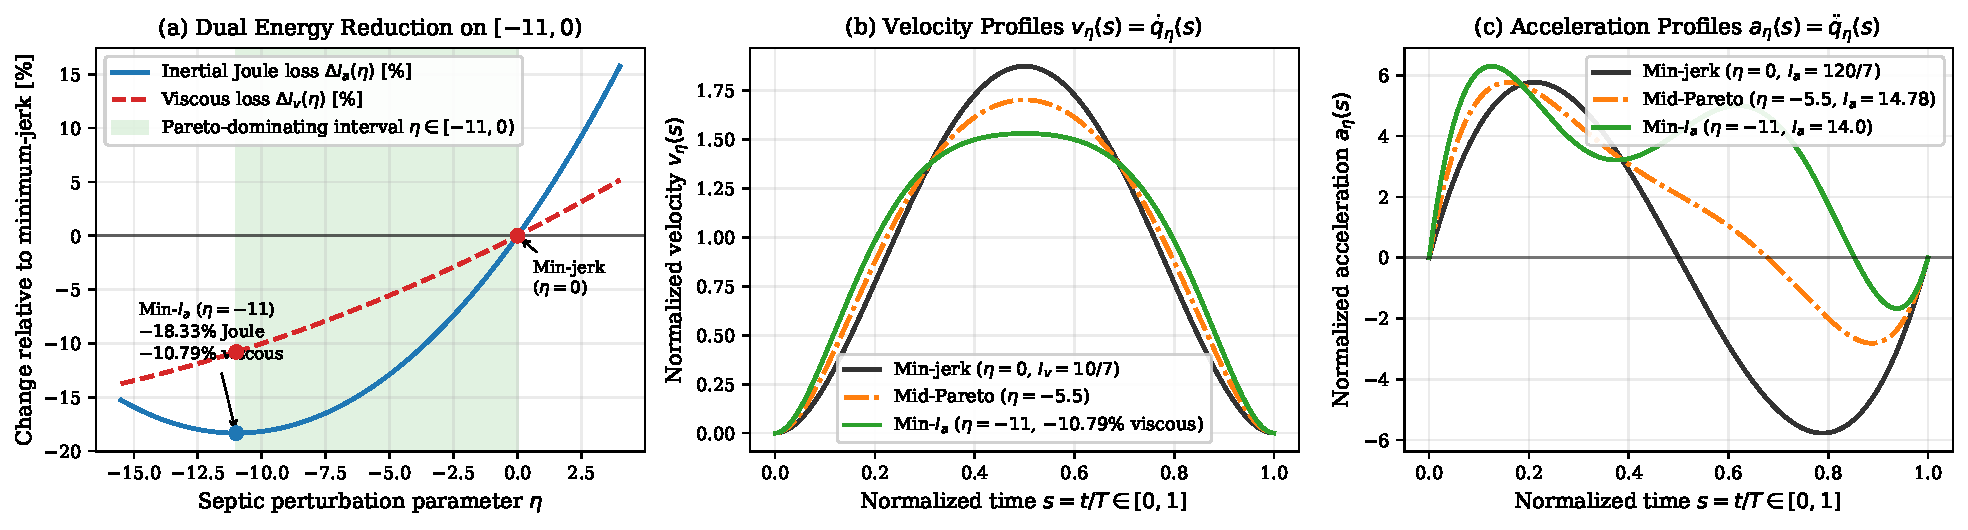
\includegraphics[width=0.98\textwidth]{figures/fig1_septic_pareto.pdf}
\caption{\textbf{Track 1 (Robotics \& Control)}: Exact polynomial antiderivative verification in \texttt{RobotEnergySmoothness.lean} showing that every septic parameter $\eta \in [-11, 0)$ strictly reduces both inertial $I^2R$ Joule loss $\int_0^T \ddot{q}^2\,dt$ (up to $-18.33\%$ at $\eta=-11$) and viscous dissipation $\int_0^T \dot{q}^2\,dt$ (up to $-10.79\%$ at $\eta=-11$) relative to classical minimum-jerk ($\eta=0$).}
\end{figure}

\begin{figure}[h!]
\centering
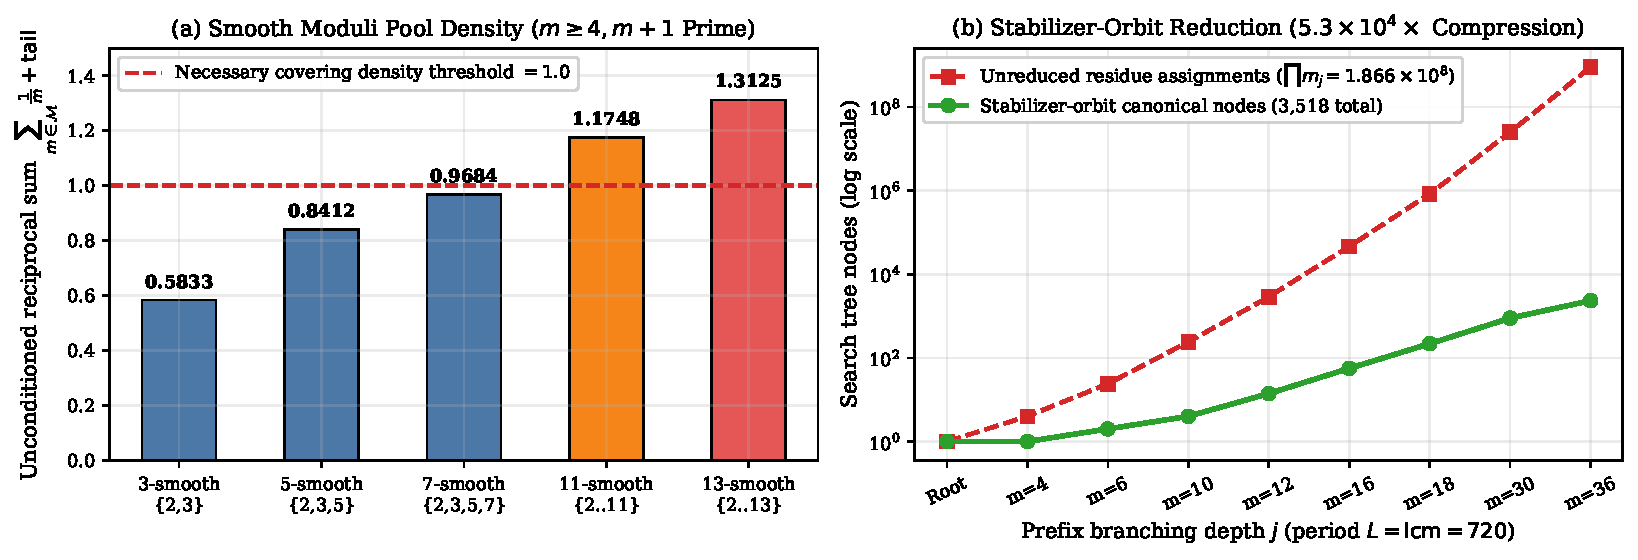
\includegraphics[width=0.94\textwidth]{figures/fig1_covering_273_tree.pdf}
\caption{\textbf{Track 3 (Experimental Math --- Erd\H{o}s 273)}: Unconditioned reciprocal density across $k$-smooth prime pools ($m \ge 4, m+1$ prime) and the $5.3\times 10^4\times$ compression achieved by stabilizer-orbit canonical branching modulo $L = \mathrm{lcm}(P) = 720$.}
\end{figure}

\end{document}
